\documentclass[11pt,a4paper]{article}
\usepackage[margin=1in]{geometry}
\usepackage{titling}
\usepackage{xeCJK}
\setCJKmainfont{AR PL UMing TW}
\usepackage{pgfplots}

\title{Virtual Machines Homework 1: Indirect Branch Handling in a Dynamic Binary Translation Based System Emulator}
\author{B01902010 李紹詮}
\date{}

\usepackage{fancyhdr}
\pagestyle{fancy}
\lhead{VM HW1}
\chead{}
\rhead{\bfseries\theauthor}
\lfoot{}
\cfoot{}
\rfoot{\thepage}
\renewcommand{\headrulewidth}{0.4pt}
\renewcommand{\footrulewidth}{0.4pt}

\begin{document}
\maketitle
\thispagestyle{fancy}

\section{Design and Implementation}
The implementation mainly follows the original function prototypes. For shadow
stack push and pop operations which are done in guest code, helper functions
are used to avoid writing TCG IR by hand, thus making the code clear to read.

\section{Experiment Results}
The Dhrystone benchmark is used for performance evaluation, and the Linux
\texttt{perf} command is used to monitor the number of branches and branch
prediction misses. Four types of implementations are tested: with no
optimization, with IBTC only, with shadow stack only, and with both
optimizations. The results are average values from 10 rounds of tests, with
10000000 Dhrystone iterations each round.

As shown in the following charts, the shadow stack has a significant performance
gain at about 32\%, reduces the number of branches at about 28\%, and reduces
about 44\% of branch prediction misses.
The performance slightly decreases when only IBTC is enabled, but it improves
performance when working together with shadow stack. IBTC also improves the
accuracy of branch prediction.

\begin{center}
    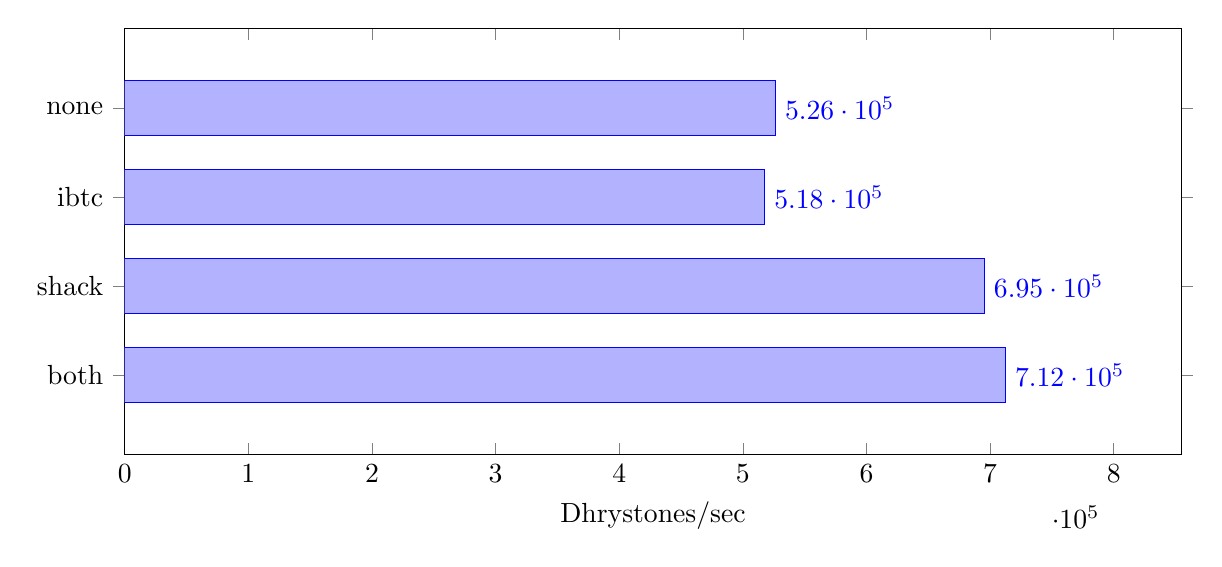
\begin{tikzpicture}
    \pgfplotsset{width=15cm, height=7cm}
    \begin{axis}[
    xbar,
    bar width=0.7cm,
    xmin=0,
    enlarge x limits={upper, value=0.2},
    enlarge y limits=0.3,
    xlabel=Dhrystones/sec,
    symbolic y coords={both,shack,ibtc,none},
    ytick=data,
    nodes near coords,
    nodes near coords align={horizontal},
    ]
    \addplot coordinates {
        (526231.7,none) (517619.3,ibtc) (695264.2,shack) (712276.1,both)
    };
    \end{axis}
    \end{tikzpicture}
\end{center}

\begin{center}
    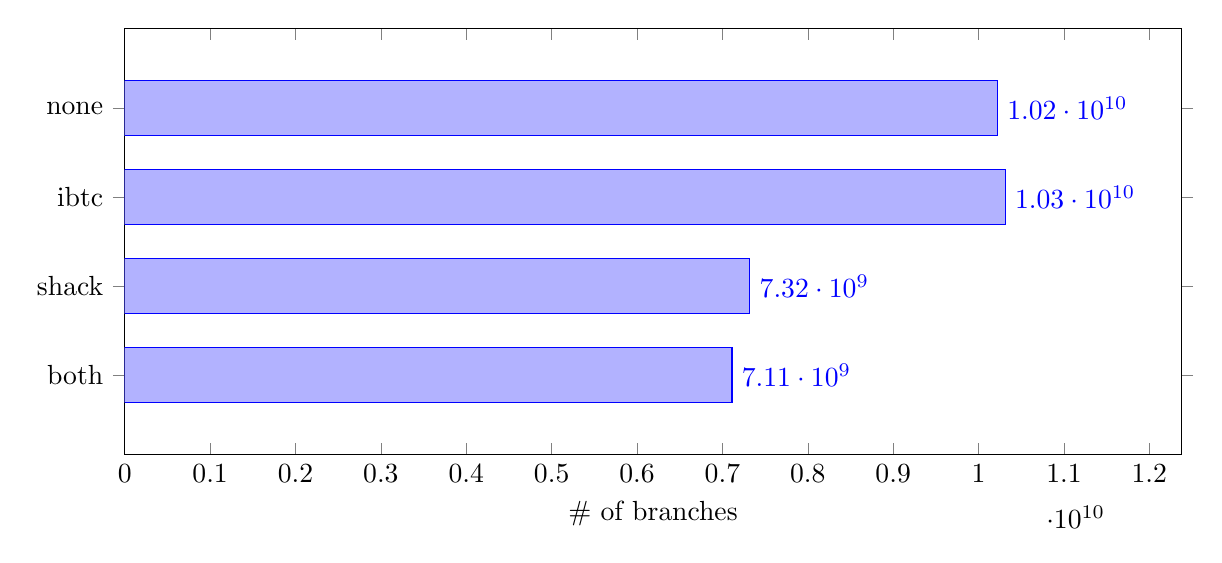
\begin{tikzpicture}
    \pgfplotsset{width=15cm, height=7cm}
    \begin{axis}[
    xbar,
    bar width=0.7cm,
    xmin=0,
    enlarge x limits={upper, value=0.2},
    enlarge y limits=0.3,
    xlabel=\# of branches,
    symbolic y coords={both,shack,ibtc,none},
    ytick=data,
    nodes near coords,
    nodes near coords align={horizontal},
    ]
    \addplot coordinates {
        (10222181842.9,none) (10312327007.4,ibtc) (7322352501.8,shack)
        (7112448224.8,both)
    };
    \end{axis}
    \end{tikzpicture}
\end{center}

\begin{center}
    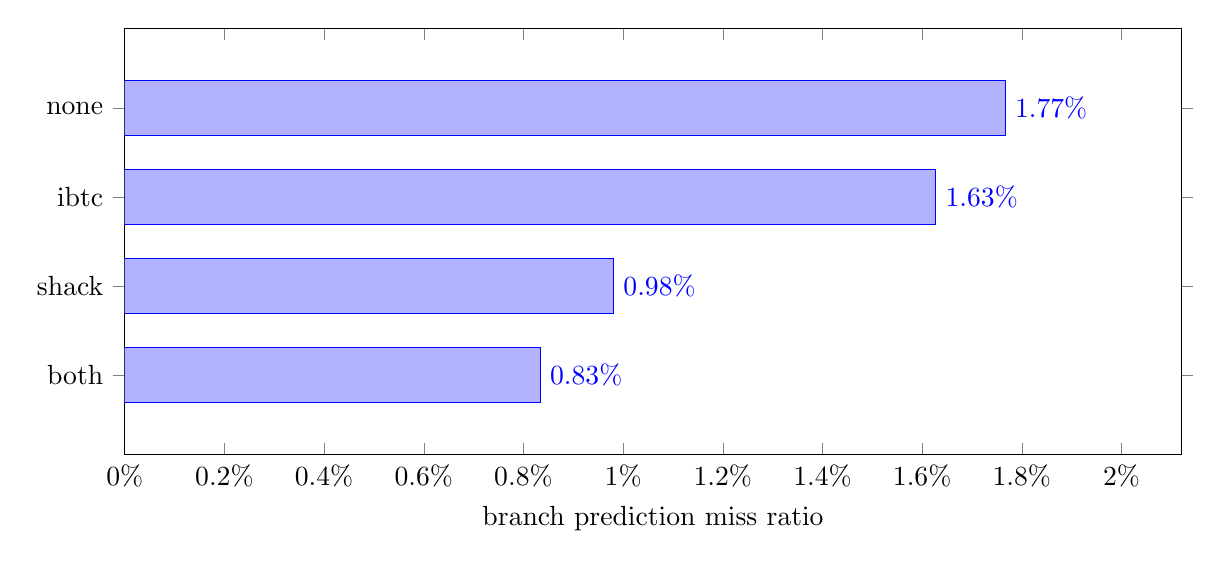
\begin{tikzpicture}
    \pgfplotsset{width=15cm, height=7cm}
    \begin{axis}[
    xbar,
    bar width=0.7cm,
    xmin=0,
    enlarge x limits={upper, value=0.2},
    enlarge y limits=0.3,
    xlabel={branch prediction miss ratio},
    scaled x ticks=false,
    xticklabel={\pgfmathparse{\tick*100}\pgfmathprintnumber{\pgfmathresult}\%},
    symbolic y coords={both,shack,ibtc,none},
    ytick=data,
    point meta={x*100},
    nodes near coords,
    nodes near coords={\pgfmathprintnumber\pgfplotspointmeta\%},
    nodes near coords align={horizontal},
    ]
    \addplot coordinates {
        (0.017667,none) (0.016275,ibtc) (0.009810,shack) (0.008338,both)
    };
    \end{axis}
    \end{tikzpicture}
\end{center}

\end{document}
